El diagrama de despliegue ilustra la arquitectura de la comunicación entre los módulos del sistema, destacando las conexiones y protocolos utilizados:
\begin{itemize}
	\item \textbf{Usuario:} Los usuarios acceden al sistema a través de dispositivos que pueden ser aplicaciones móviles (App) o navegadores web (Browser). La comunicación se realiza mediante el protocolo HTTPS en el puerto 443 para garantizar la seguridad de los datos transmitidos.
	\item \textbf{Servidor Web:} Este componente, desplegado en la nube, aloja la página web de la aplicación. Se encarga de servir las interfaces de usuario y manejar las solicitudes HTTPS provenientes de los clientes.
	\item \textbf{Servidor (AWS EC2):} El servidor principal está desplegado en un servicio EC2 de AWS. Este servidor maneja la lógica de negocio y procesa las solicitudes de los usuarios, comunicándose con la base de datos para acceder y manipular la información necesaria.
	\item \textbf{Base de Datos (MongoDB Atlas):} La base de datos está alojada en MongoDB Atlas, un servicio de base de datos en la nube. Este componente almacena todos los datos del sistema, organizados en esquemas como “Actividades” y “Usuarios”. La comunicación entre el servidor y la base de datos se realiza a través de una URI segura.
\end{itemize}

El diagrama también muestra cómo el servidor web y el servidor principal (EC2) se comunican con la base de datos en MongoDB Atlas.

\begin{figure}[H]
	\centering
	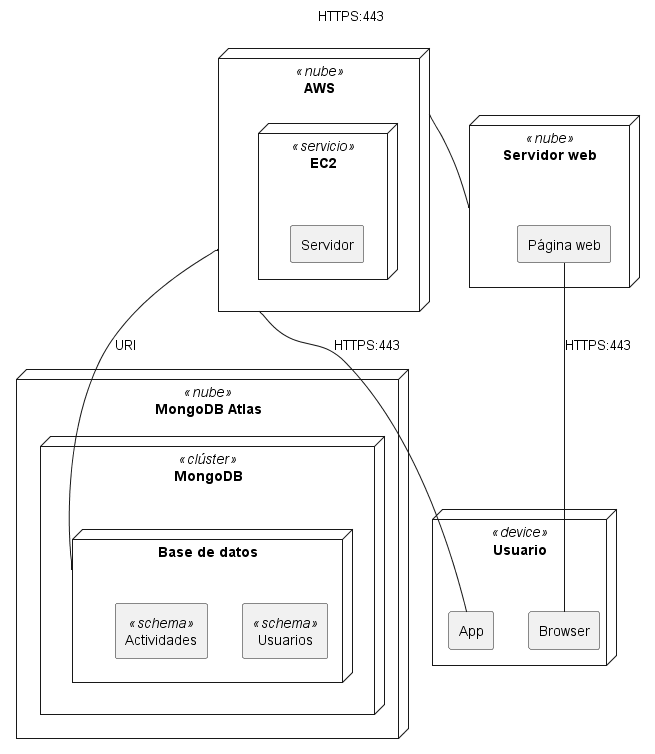
\includegraphics[width=1\linewidth]{6-DiseñoDelSistemaDeInformacion/Modulos/comunicaciones.png}
	\caption{Diagrama de despliegue}
\end{figure}